\documentclass[13pt]{article}
\usepackage[margin=1in]{geometry}

% The preceding line is only needed to identify funding in the first footnote. If that is unneeded, please comment it out.
\usepackage{cite}
\usepackage{amsmath,amssymb,amsfonts}
\usepackage{algorithmic}
\usepackage{graphicx}
\usepackage{textcomp}
\usepackage{xcolor}
\usepackage{setspace}
\usepackage{hyperref}
\onehalfspacing
\def\BibTeX{{\rm B\kern-.05em{\sc i\kern-.025em b}\kern-.08em
    T\kern-.1667em\lower.7ex\hbox{E}\kern-.125emX}}

% \parindent=0pt

\begin{document}


\begin{titlepage}
\enlargethispage{1cm}

\begin{center}

\textbf{\Large \uppercase{Predicting Distant Metastasis Survival Function in Breast Cancer using COBRA}}
 
 \vspace{2cm}
 
A Project Report Submitted \\
for the Course \\[1cm]

{\bf\Large\ MA691 Advanced Statistical Algorithms }\\[.1in]
{\Large\ Asst. Prof. Arabin Kumar Dey }\\[.1in]

\vspace{2cm}

{\large \emph{by}}\\[5pt]
{\large\bf {Adit Jain}} {\large (180102003)} \\
{\large\bf {Kousik Rajesh}} {\large (180101094)} \\ 
{\large\bf {Eklavya Jain}} {\large (180123065)} \\
{\large\bf {Drishti Chouhan}} {\large (180101021)} \\ 
{\large{J. Neeraja}} {\large (180123017)} 

\vspace{3cm}

\includegraphics[height=2.5cm]{images/iitglogo.eps}

{\em\large to the}\\[10pt]
{\bf\large DEPARTMENT OF MATHEMATICS} \\[5pt]
{\bf\large \mbox{INDIAN INSTITUTE OF TECHNOLOGY GUWAHATI}}\\[5pt]
{\bf\large GUWAHATI - 781039, INDIA}\\[10pt]
{\it\large November 2021}
\end{center}

\vspace{1cm}


\textbf{DISCLAIMER:} This work is for learning purposes only. The work can not be used for publications or commercial products etc. without mentor's consent. 

\end{titlepage}

\normalsize
\begin{center}
\Large
\textbf{Abstract}
\end{center}
Metastatic Breast Cancer can develop when breast cancer cells break away from the primary tumor and enter the bloodstream or lymphatic system. Metastases are the primary cause of death of cancer patients, and improving the means of foretelling their development is a major goal of current clinical research. Here we analyse the TRANSBIG dataset and obtain the gene signatures of 198 breast cancer patients along with their characteristics. We predict the survival function for distant metastasis of lymph-node-negative primary breast cancer using multiple regression models and combining their predictions using COmBined Regression Alternative (COBRA). We compare our findings with the existing ensemble learning technique, Random Survival Forest, and reported the accuracy score for both methodologies. We report an improved accuracy of 0.78 in comparison to 0.57 offered by the Random Survival Forest. We also present our pipeline to predict the time for distant metastasis, which can be further extended to apply COBRA Technique on any healthcare dataset.


% \begin{IEEEkeywords}
% COBRA, Multivariate Analysis, Breast Cancer Metastatis, Machine Learning
% \end{IEEEkeywords}


\clearpage

\section{Literature Review}
\subsection{TRANSBIG dataset}
Gene signatures of cancer patients have been extensively used in clinical research to predict distant cancer metastasis. There have been regressive attempts to accurately predict diagnosis and treatment for these patients by analysing appropriate gene expression data. One such instance is the research corpus that uses the TRANSBIG dataset(Gene expressions of 198 systematically untreated patients) to predict distant metastases in lymph node-negative (N-) breast cancer patients. Several methodologies have been used overtime to improve the accuracy of predictions and understand the genetics that influences these prognostics. The research pipeline consists of the following steps: 
\begin{itemize}
    \item Correctly identifying the appropriate gene signature that is relevant to breast-cancer. 
    \item Validating the performance of the 76-gene signature to support the growing evidence that gene expression signatures are of clinical relevance, especially for identifying patients at high risk of early distant metastases.
    \item Performing a better gene-selection, eg. feature selection to select 12 genes which showed a higher area under the receiver operating characteristic curve of 0.730 compared with 0.579 yielded by previously reported 76 genes.
    
\end{itemize}

\subsection{Identifying 76-gene signature for predicting metastatis} 
22,000 gene-transcripts from the RNA 286 lymph-node-negative patients who had not received systemic treatment, was analysed. In a training set of 115 tumours, 76-gene signature consisting of 60 genes for patients positive for oestrogen receptors (ER) and 16 genes for ER-negative patients was identified. This signature showed 93\% sensitivity and 48\% specificity in a subsequent independent testing set of 171 lymph-node-negative patients. The methodology adopted was as follows: 
\begin{enumerate}
    \item 17,819 genes were 'present' in two or more samples and were eligible for hierarchical clustering. 
    \item To identify genes that discriminated patients who developed distant metastases from those remaining metastasis-free for 5 years, two supervised class prediction approaches were used. The first being randomly building a training dataset of 80 and testing dataset of 206 patients. Kaplan-Meier survival curves for the two sets were examined to ensure that there was no significant difference. The second approach was to randomly allocate patients to one of the two subgroups based on Er status. 
    \item Univariate and multivariate analyses with Cox’s proportional-hazards regression were done on the individual clinical variables with and without the gene signature. The hazard ratio and its 95\% CI were derived from these results.
    \item After 5 years, absolute differences in distant-metastasis-free and overall survival between the patients with the good and poor 76-gene signatures were 40\% and 27\%, respectively.\cite{wang2005gene}
\end{enumerate}

\subsection{Validating the prognosis signature} 
A study conducted by TRANSBIG to validate the 76-gene prognostic signature for distant metastasis and compare the results with clinical risk assessment. The results of this experiment showed that there was a strong time dependence leading to an adjusted hazard ratio of 13.58 (1.85-99.63) and 8.20 (1.10-60.90) at 5 years and 5.11 (1.57-16.67) and 2.55 (1.07-6.10) at 10 years for time to distant metastasis and overall survival, respectively.\cite{desmedt2007strong}

\subsection{Correlation-centred gene selection to reduce gene-set} 
A robust feature-selecting strategy with a correlation-centred approach to select minimal gene sets was developed using a multiple logistic regression model. This method selected 12 genes which showed a higher area under the receiver operating characteristic curve of 0.730 compared with 0.579 yielded by previously reported 76 genes. In conclusion, a smaller gene-set that has higher predictive capabilities and increased applications in cancer-treatment has been identified. There have been various other methods explored as described below which can be used to improve the ROC.\cite{hikichi2020correlation}

\subsection{Different machine-learning and deep-learning models on \\TRANSBIG} 
One of the many approaches was an Ensemble machine learning technique\cite{zakharov2011ensemble} that combines multiple classifiers to improve performance by choosing feature subsets and learning predictive models. \\
DeepProg\cite{poirion2019multi}, is another novel ensemble framework of deep-learning and machine-learning approaches that robustly predicts patient survival subtypes. DeepProg is highly accurate, with a c-index of 0.68-0.73. \\\\Other papers \cite{djebbari2008ensemble} ,\cite{jiao2015kendall}, \cite{mirsadeghi2019post} have also analysed the TRANSBIG dataset and made significant contribution to improve predictive performance but none have explored the impact of Combined Regression on the same. 

\subsection{COBRA}
Multiple initial estimators of the regression function can be combined, instead of building a linear or convex optimized function over a selection of basic estimators. This can be used as a collective indicator of the proximity between training data and test results. This local-distance approach is fast and efficient, which  performs asymptotically in the L\textsuperscript{2} sense as the best combination of the basic estimators in the collective. The increased accuracy and reduced Brier-score of the COBRA strategy can help achieve better classifier performance on the TRANSBIG dataset.  \cite{biau2016cobra}




\section{Brief overview}
To predict the survival function for distant metastasis we initially create indicator variables for time instances ranging from 0 to 8000 days with a step size of 100 days, and add them as separate columns in the dataset. Each of these columns denote if metastasis has occurred until a certain point. These indicator variables are binary variables and are estimated by applying classification models on the training data. Subsequently, these columns are combined to estimate the survival function. We train different classification models such as Support Vector Classifier, K Nearest Neighbours Classifier, Logistic Regression, Gaussian Naive Bayes and Linear Discriminant Analysis each of which output a value between 0 and 1 denoting the probability of the indicator variable being true. For each indicator variable, we then combine these predictions through a Combined Regression (COBRA) Strategy. Our COBRA technique is soft in nature, meaning rather doing a hard match for each data point of the the test dataset, it combines the predictions using an epsilon threshold. This epsilon parameter used by COBRA is a measure of the selectivity of the model and we perform a grid search with brier score as the scoring function to choose the optimal value of epsilon. We benchmark our results by comparing the average accuracy obtained by COBRA over all indicator functions with the average accuracy obtained by logistic regression, Random Survival Forest and a simple average over models. We achieved an accuracy of $0.78$ in comparison to Random Survival Forest's accuracy of $0.57$.
\section{Methodology}

\subsection{Dataset}
The dataset for this project was obtained from the original study conducted by TRANSBIG to test the possibility of predicting distant metastases in lymph node-negative breast cancer patients using 76-gene signature's ability. Gene Expression profiling was done from frozen samples of 198 node negative untreated patients.  \footnote{The dataset is publically available online at https://www.ncbi.nlm.nih.gov/geo/query/acc.cgi?acc=gse7390} The dataset has three aspects, gene expression, clinical data and genomic risk which are obtained independent to each other. The gene expression contains expressions data for 22283 genes, out of which only 76 are relevant for breast cancer metastatis prediction, which are extracted. The clinical data contains various attributes of the patient, importantly the age, size of tumor, time to distant metastasis and censoring variables for the same. The genomic risk are different diagnostic risks including the NPI Score, score by Adjuvant Online (AOL) and Veridex, and Clinical Risk Group by St. Gallen Criteria. These datasets are extracted and combined for each of the 198 patients to create a single dataset. 




\subsection{Train-Test split}
For performing our model analysis we split the dataset into training and testing data using a split ratio of 0.66 and doing a random split. This gives us 118 data points in the trainset and 70 in the test set. This split has been taken because the initial number of data points is itself very small, and to get some statistically significant results we need enough test data points.   

\subsection{Creating intermediate variables}
We create 80 indicator variables which act as intermediate variables for time points ranging from 0 days to 8000 days that denote the event that metastasis has taken place. This indicator variables are spaced at distance of 100 days each.\\


The equation for creating an indicator variable at time point $T$ is $I_{t < T} = 1$ if time to distant metastasis is less than the value T, otherwise 0.\\


The intermediate variables that were created are used later on used to approximate the cummulative survival function since predicting the survival function is otherwise not possible. The indicator functions are predicted using the approach highlighted below. \\

\subsection{Estimating intermediate variables}
We use estimators especially COBRA (explained below) to predict each of these indicator variables. When working on the test data we use the trained model to generate predictions in the form of probabilities for each indicator variable. We then combine these estimated indicator functions to form the survival function. 

\subsection{Calculation of survival function}
The survival function is calculated using the indicator variables that we predicted in the last step. The equations for calculation are detailed below $$S(t) = Pr\{T \geq t \} = 1 - F(t) = \int_t^{\infty}f(x)dx$$
Here $F(t)$ is the cumulative probability that metastasis has occurred, in our case the predictied probability of the indicator function at point $t$ serves as an estimate for $F(t)$.

\subsection{Combined Regression Strategy (COBRA)}
\subsubsection{Introducti           on to COBRA}
COBRA which stands for Combined Regression is a method used to combine multiple weak learners. Given a set of preliminary estimators $r_1, .. , r_M$, the idea behind this combining method is an unanimity concept. It creates a prediction mapping for each weak learner on the training data. These are then used while predicting on the test data to find existing datapoints that are close to the considered point. The prediction corresponding to these datapoints are used to generate the final prediction by taking help of some summary metric (Mean in our implementations). 

\subsubsection{Overview of model}
We first split the training dataset into two groups of equal sizes, and then our implementation initializes different models to predict the indicator functions. These models are trained using one of these halves and the models predict the indicator function over the other half.  These prediction results are stored for each of these models and are used for predicting outcomes, these are referred to as reference-training data. For predicting the indicator outcome for an input from the test data, we do the following:
\begin{itemize}
    \item For each machine, we find its prediction on the considered test point and we iterate through the prediction table to find $\epsilon$ close predictions. We mark these predictions for those machines
    \item We pick up the reference-training data points which have all machines giving $\epsilon$ close predictions (The total number of machines/models is given as $\alpha$) 
    \item Taking the mean of prediction probabilities corresponding to these data-points, which we already have since this is the training data, we get the outcome corresponding to our required test data point.   
\end{itemize}

\subsubsection{Constituent classification models}
\hspace{0.5cm}\begin{itemize}
    \item \textbf{Support Vector Classifier} - The Support Vector Classification algorithm builds a model that assigns new examples to one category or the other, making it a non-probabilistic binary linear classifier.
    \item \textbf{K Nearest Neighbours Classifier} - The KNN classification algorithm uses a distance metric to find k closest neighbors of a given test point and classifying it into the majority class.
    \item \textbf{Decision Tree Classifier} - The Decision Tree Classifier builds a Decision tree to classify samples into different classes.
    \item \textbf{Logistic Regression} - Logistic Regression which is actually a classification algorithm generates a decision boundary between two classes based on the training data.
    \item \textbf{Gaussian Naive Bayes} - Gaussian Naive Bayes is a model based on Bayes’ Theorem and has a strong assumption that predictors should be independent of each other. 
    \item \textbf{Linear Discriminant Analysis} - LDA is closely related to principal component analysis (PCA) and factor analysis in that they both look for linear combinations of variables which best explain the data.
    
We use these models as a constituent model with the default hyperparameters provided by sklearn.
\end{itemize}
\subsubsection{Metrics for evaluation}
\begin{itemize}
    \item \textbf{Brier Score} - Brier score is a strictly proper scoring rule that measures the accuracy of probabilistic predictions. The Brier score is calculated as follows:
    Across all items $i \in 1..N$ in a set of N predictions, the Brier score measures the mean squared difference between: the predicted probability assigned to the possible outcomes for item $i$ and the actual outcome.
    $$BS = \frac{1}{N}\sum\limits _{t=1}^{N}(f_t-o_t)^2 $$
    Here $f_{t}$ is the probability that was predicted, $o_{t}$ is the actual outcome of the event at instance $t$ ($0$ if it does not happen and $1$ if it does happen) and $N$ is the number of predicting instances. 
    \item \textbf{Accuracy} - The accuracy score is the percentage of labels predicted that match the corresponding set of true labels in the evaluating dataset.


\end{itemize}
\subsubsection{Finding optimal epsilon}
Epsilon as discussed earlier is used to control the selectivity of the COBRA model, this epsilon can take real values within the range of 0 to 1, Values near to 0 signifying a highly selective model. This epsilon can be hard coded to a particular value but that prevents the possibility of improving the model. And so to find the optimal value, cross validation is done on the training set using a continuous range of different epsilons, this technique is often referred to as grid search in optimization literature. For each value of epsilon, we calculate the brier score for a subset of the training data. The epsilon corresponding to the minimum brier score is taken to be the optimal epsilon is then used to run the final model on the test data-set for each of the indicator functions to finally obtain the survival function shown in Results.  
\subsection{Random Survival Forest}
Random Survival Forests are a class of Random Forests which were introduced for specific analysis of right censored data and are used in predicting different kinds of survival metrics, including mortality, survival function and hazard function. A basic overview of the random survival function can be given as: 
\begin{itemize}
    \item Drawing B bootstrap samples from the original data
    \item Growing a survival tree for each of the bootstrap sample, at each node of the tree $p$ candidate variables are selected. The node is then split using the candidate variables that maximizes the survival difference between daughter nodes. 
    \item The tree is grown to full size until the constraint that any terminal node doesn't have less than $d_0 > 0$ deaths.
    \item A CHF is calculated for each tree and an average of all CHFs is taken as the ensemble CHF
    \item Using out-of-bag data a prediction error is calculated
\end{itemize}

\section{Implementation and Results}

The experiments were conducted in python with the help of libraries like Scikit-Learn, Scikit-Survival, Numpy, Pandas, and Matplotlib. Scikit-Learn was used to train classification models like Support Vector Classifier, K Nearest Neighbors, Decision Tree Classifier, Logistic Regression, Gaussian Naive Bayes, and Linear Discriminant Analysis. Furthermore, Sklearn metrics like accuracy, brier score, and RMSE were used. \\

The experiment is executed on a system having the following configuration: \\
(i) Intel\textsuperscript{\tiny\textregistered} Core\textsuperscript{\texttrademark} i5-8250U CPU @ 1.60GHz x 4, (ii) Ubuntu 20.04 LTS OS, and (iii) 12 GB Memory. \\

The 76 gene features along with the age, size, NPI score and Adjuvant Online (AOL) were considered as the explanatory variables, and the constructed indicator variables for time to distant metastasis as the response variable. \\

The predictions of the indicator variables were extended to calculate the survival function, and further the cumulative hazard function. The graphs for both the survival function and the cumulative hazard function are plotted for our native implementation of COBRA as well as Random Survival Forest present in Scikit-Survival library. Figure \ref{fig:haz} plots the cumulative hazard function of 5 patients against time in days for our native implementation of COBRA. Figure \ref{fig:hazpy} plots the same function calculated using Random Survival Forest. Figure \ref{fig:surv} plots the survival function of the same 5 patients against time in days for our native implementation of COBRA. Figure \ref{fig:survpy} plots the same function calculated using Random Survival Forest. 

\begin{figure}[h!]
    \centering
    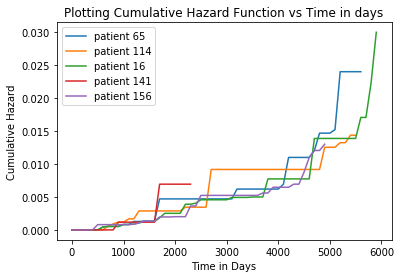
\includegraphics[width = 0.65\textwidth]{images/haz.png}
    \caption{Cumulative Hazard Function of 5 patients on applying COBRA }
    \label{fig:haz}
\end{figure}

\begin{figure}[h!]
    \centering
    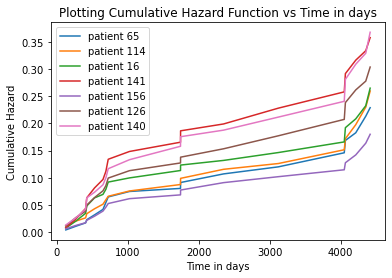
\includegraphics[width = 0.65\textwidth]{images/hazpy.png}
    \caption{Cumulative Hazard Function of 5 patients on applying Random Survival Forest}
    \label{fig:hazpy}
\end{figure}

\begin{figure}[h!]
    \centering
    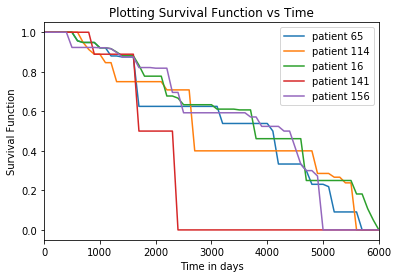
\includegraphics[width = 0.65\textwidth]{images/surv.png}
    \caption{Survival Function of 5 patients on applying COBRA }
    \label{fig:surv}
\end{figure}

\begin{figure}[h!]
    \centering
    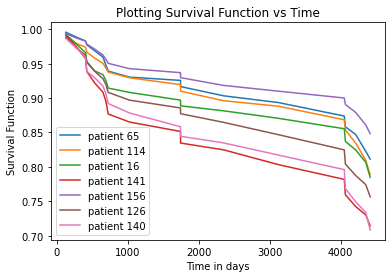
\includegraphics[width = 0.65\textwidth]{images/survpy.png}
    \caption{Survival Function of 5 patients on applying Random Survival Forest}
    \label{fig:survpy}
\end{figure}

In Figure \ref{fig:acc_comp}, we compare the accuracies offered by various models. In figure \ref{fig:brier} we compare the brier score corresponding to each model. We see that our method (using COBRA) provides the best accuracy and the least brier score among all the machines, even Random Survival Forest. 

\begin{figure}[h!]
    \centering
    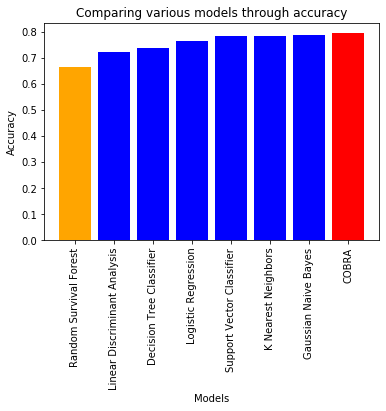
\includegraphics[width = 0.5\textwidth]{images/acc_comp.png}
    \caption{Comparison using Accuracy of various models used in our Analysis}
    \label{fig:acc_comp}
\end{figure}

\begin{figure}[h!]
    \centering
    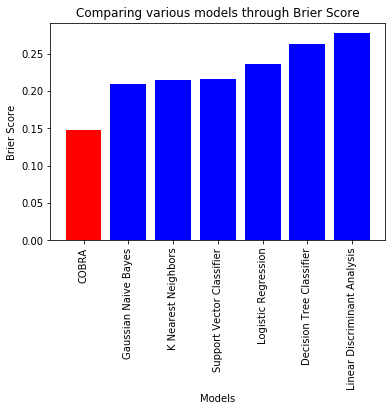
\includegraphics[width = 0.5\textwidth]{images/brier_score.png}
    \caption{Comparison using Brier Score of various models used in our Analysis}
    \label{fig:brier}
\end{figure}

% Comparison ofaccuracies with other models
% Survival and hazard function of cobra and rsf
\pagebreak
\clearpage
\nocite{*}
\bibliographystyle{apalike}
\bibliography{cobra_report}
\end{document}
